\section{Optical Receiver Payload}
	\label{blDOreceiver}
		\subsection{Introduction}
A large fraction of the photons emitted by the \acs{laser} are not suitable for detection since they are redirected by the atmosphere, spread due to surface scattering or they are simply absorbed by either of them. The decrease in photon quantity is really severe considering these factors. Since the number of photons actually reaching the perimeter of the \ac{ORD} are usually only in the order of one to ten, the \acs{ORD} has to be able to detect and analyze individual small energy packets, preferably single photons. 

The main objective of the \acs{ORD} in that sense is to detect the individual energy quanta. An obvious way of achieving this is to increase the \acs{ORD} receiving surface area. In this case, more photons can be detected which normally, with a relative small optical receiving area, would go passed the receiver. The main disadvantage is the increase in noise, which decreases the quality of your measurements. The \acs{laser} used in this altimetry mission is not the only electromagnetic radiation source in the neighborhood of the satellite constellation. Next to thermal radiation from Earth, electromagnetic radiation from other celestial objects and other spacecraft, the Sun is also a major contributor of electromagnetic radiation. All of these sources are considered irrelevant to the altimetry mission and therefore, can be categorized as noise. Increasing the \acs{ORD} receiving area consequently increases the detection of noise. An optimal receiving-surface-area to noise-detection ratio should be determined.

\subsection{Types of Optical Receiving Devices}
	\label{blDOtypesORD}
The science behind single photon detection is a relative new branch in the field of quantum optics and at the moment, considering its capabilities and myriad applications, the amount of research done in this field is growing by the day. A number of technologies, primarily based on quantum dynamics, and devices are already in production or in development. Since the science behind the single photon detection devices is pretty elaborate, only an introduction of the techniques are given below.

\begin{enumerate}[i]
	\item \ac{CCD}. A \acs{CCD} is a two-dimensional array of metal-oxide-semiconductor capacitors which can accumulate and store charge due to their capacitance. When the device is properly biased, the electrons in each array element 'feel' a finite potential well in which they are trapped, assuming no quantum tunneling, i.e. no motion of electrons through potential barriers. By inducing energy to these trapped electrons, the energy can exceed the potential barrier well. If the capacitors and the electrons are in thermal equilibrium, this induced energy should come from photonic excitation (assuming no applied external electric field). If a photon with the proper wavelength (and hence with the proper amount of energy) hits one of the capacitors, electron excitation can occur, giving it an energy level higher than the energy of the potential well. Of course, the energy of the incoming photon should be equal or higher than the energy difference of the initial electron state and the potential energy. Once the energy of the electron is beyond the potential energy, a charge is created which can be measured by applying a PN-junction structure in cooperation with the two-dimensional array. 
	
Usually, the number of photons actually hitting one specific capacitor is not equal to one. Single photon detection however could be achieved by registering individual photonic excitations per capacitor. 

The main advantage of \acs{CCD}s is the high level of technical readiness and the fact that a single capacitor failure does not influence the overall performance.

\item Photomultiplier Tubes (Avalanche Processes). Photomultiplier tubes are photon detectors that are useful in low intensity applications. A photomultiplier tube is a vacuum tube consisting of an input window, a photocathode, focusing electrodes, an electron multiplier and an anode.
Figure \ref{Photomultiplier} on page \pageref{Photomultiplier} gives a clear view of photomultiplier tube configuration and working mechanism.
\begin{figure} [h]
	\begin{center}
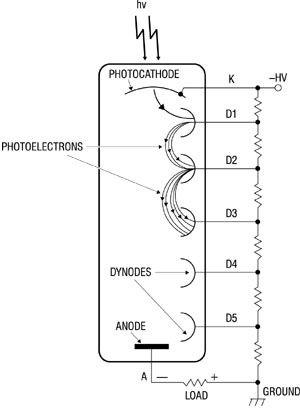
\includegraphics[scale=3]{chapters/img/DO_receiver1.jpg}	
\caption{Photomultiplier tube configuration and working mechanism}
\label{Photomultiplier}
\end{center}
\end{figure}

The main mechanism of this device actually uses the photoelectric effect, which refers to the emission, or ejection, of electrons from the surface of, generally, a metal in response to incident light. Energy contained within the incident light is absorbed by electrons within the metal, giving the electrons sufficient energy to be 'knocked' out of, that is, emitted from, the surface of the metal. Next to this emission of the electron, secondary emission is induced due to the appliance of an electric field into the tube, giving the incoming electrons more energy. This way, the number of electrons increase with dynode bypass. 

The main disadvantage is that a single tube measures one photon at a specific time. Making a array of tubes adds a lot of mass to the overall system. 

\item Quantum Dots. Quantum dots are semiconductor nanocrystals having dimensions in the order of 2 - 50 nanometers. A semiconductor is a material that has a small bandgap between the valence and conduction band. An exciton pair is defined as an negatively charged electron and the positively charged hole it leaves behind when it is excited up to the conduction band. The exciton-Bohr radius is equal to the exciton distance. A quantum dot is a semiconductor so small that the size of the crystal is on the same order as the exciton-Bohr radius, giving birth to small number of quantized discrete energy levels. 

The \acs{QDRD} is based upon a transistor structure in which the conducting channel is closely spaced from a layer of quantum dots. If the separation of the quantum dots and the channel is just several nanometers, the resistance of the transistor is sensitive to a change in the occupancy of a single quantum dot by just a single electron. This attribute allows the device to act as a detector of single photons, since the absorption of a photon creates carrier in the semiconductor, which after capture by a quantum dot, produce a detectable change in the resistance of the channel of the resistor.
\ref{quantumdots}

MPS's single-photon detection modules (see Design Option Tree) uses quantum dots.
Figure \ref{quantumdot} on page \pageref{quantumdot} gives a clear view of single photon detection using quantum dot configuration.
\begin{figure} [h]
	\begin{center}
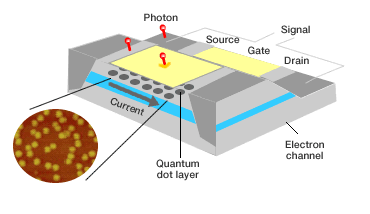
\includegraphics[scale=1]{chapters/img/blDOreceiverQDRD.png}	
\caption{Single photon detection using quantum dot configuration}
\label{quantumdot}
\end{center}
\end{figure}

\item Quantum Computers. Quantum computers use, in contrary to regular computers, no semiconducting chips for processing. Although this technology is very interesting with myriad possibilities, the technology behind it is not understood very well at this point. Scientist are mainly focusing on the theory behind it, without actually building a (theoretical first) model. Although futuristic, many scientists predict a bright future for quantum computers in the field of optics.

Basically, the theory behind quantum computers relies on intrinsic properties of fermions. Fermions are elementary particles with a specific value of intrinsic spin (not angular momentum about principal axis). Fermions, like electrons, have a specific intrinsic spin of 1/2. This spin can be spin up (+1/2) or spin down (-1/2). Pauli's exclusion principle states that no identical fermion can exhibit the same energy level, i.e. two electrons can occupy one energy orbit (spin-up and spin-down). Electromagnetic radiation can alter spin configurations. By evaluating spin characteristics, a binary code could written.
\ref{quantumcomputers}
	
\end{enumerate}

\subsection{Important parameters for optical receiving devices}
	\label{blDOparametersORD}
Obviously, the mass and the average power usage are important aspects for choosing the desired \acs{ORD} in any satellite (constellation) mission. 

Considering the fact that you want to detect as much photons as possible, another important characteristic is the \ac{OFOV}. The \acs{OFOV} (also field of vision) is the (angular or linear) extent to which the \acs{ORD} is able to observe photons at any given moment. As mentioned earlier, the problem of noise increases if the \acs{OFOV} becomes too large. However, since the \acs{OFOV} is in the order of 0.001 radians, it can be stated that a higher values increases the detectable photons.

The last aspect to consider when determining the \acs{ORD}, is the detector quantum efficiency. Basically it is defined as the efficiency that an incoming photon induces an exciton. It is an accurate measurement of the device's electrical sensitivity to light. 
Figure \ref{DOS_receiver} on page \pageref{DOS_receiver} gives the final design option tree of the laser receiver.
\begin{figure} [h]
	\begin{center} 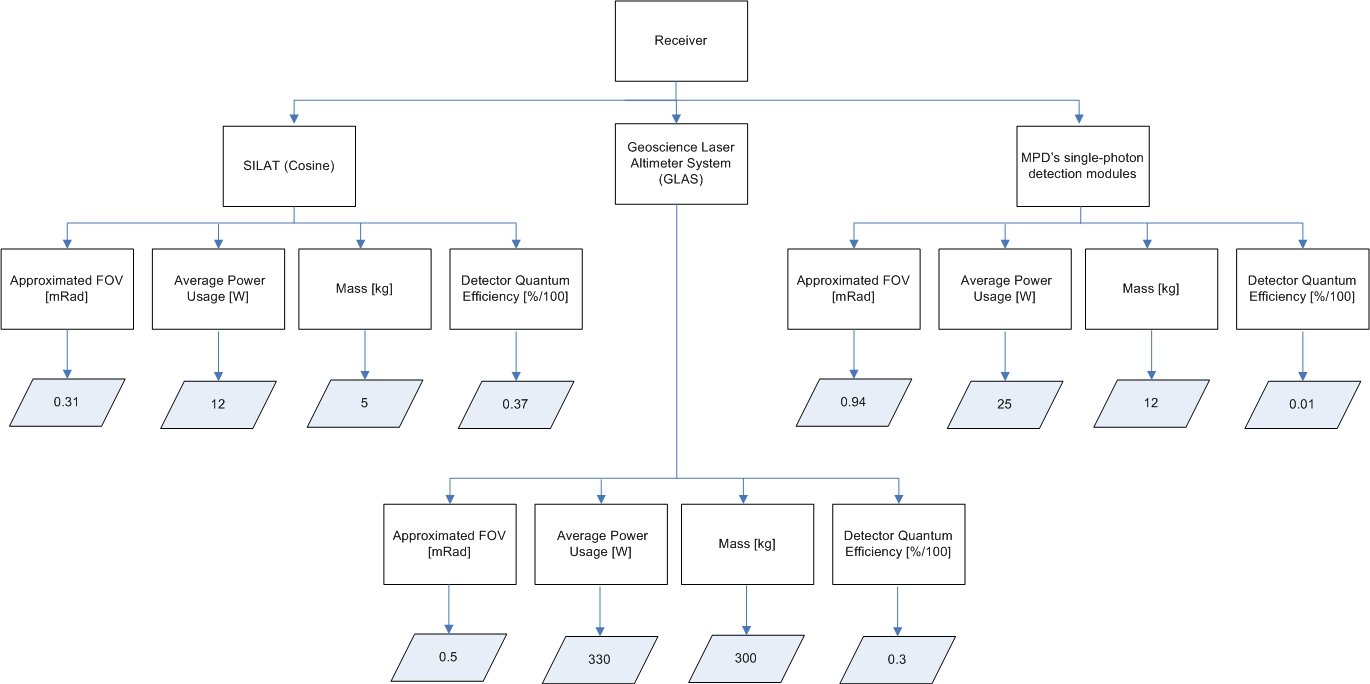
\includegraphics[width=1\textwidth,angle=90]{chapters/img/DOStree_receiver.jpg}	
	\caption{Design option tree of laser receiver}
	\label{DOS_receiver}
	\end{center}
\end{figure}